\section{Comparison of models}\label{sec:evaluation-models}

% parameters
Similar to \citeauthor{glove2014}'s work, in this thesis, for many models used, any unspecified parameters are set to their default values, 
assuming that they are close to optimal
acknowledging that this simplification should be revised in a more thorough analysis.

% comparing models (qualitative)
This evaluation does not aim to find the best model but to compare the similarity of the models' query results.
It is a qualitative evaluation of a selection of documents from the Bahamas leak.
This selection is a 2048 document corpus that was randomly chosen without replacement.
A query defines a field, i.e. embedding model and a query document.
The query response consists of the documents that are considered most similar to the model's embedding of the query document in terms of cosine similarity.
These responses are retrieved by a \ac{knn} query from the database for each model and stored in a \ac{csv} file.
To facilitate working with the data, the document IDs can be encoded as monotonically increasing integers.

% Venn diagram
The first approach to compare the response documents is to visualize the intersection of the query results.
The Venn diagram was chosen since it displays intersections of all items of the power set of the models.
To build a Venn diagram, the number of documents that are shared between the query results of several models is computed.
First, all query responses of a model irrespective of the query document are saved in a set.
The cardinalities of the intersections of multiple sets are displayed in \autoref{fig:venn-comparison-models}.
Since five models encode textual information the Venn diagram consists of five circles.
One should be cautious when interpreting the layout of the Venn diagram since 
an intersection of documents that produces an empty set has a non-empty area in this visualization.

The Venn diagrams in \autoref{fig:venn-comparison-models} display the total number of shared response documents for 10 queries 
and 3, 5 or 10 response documents respectively.
The models produce rather dissimilar query results.
Any combination of more than two models among the green (\ac{d2v}), orange (\ac{sbert}), red (\ac{tfidf}) and blue (\ac{use}) models 
seem to produce rather dissimilar results 
as the number in the respective areas at the bottom is close to zero across all Venn diagrams.
The blue (\ac{use}) and orange (\ac{sbert}) models, as well as the yellow (\infersent{}), orange (\ac{sbert}) and blue (\ac{use}) models, 
yield consistently similar results.

\begin{figure}%
    \centering
    \subfloat[\centering 3 response documents per query.]{{\includegraphics[width=6.7cm]{images/comparison/Venn_diagram_(10_queries_à_3_responses_in_a_2048_document_corpus).pdf} }}%
    \qquad
    \subfloat[\centering 5 response documents per query.]{{\includegraphics[width=6.7cm]{images/comparison/Venn_diagram_(10_queries_à_5_responses_in_a_2048_document_corpus).pdf} }}%
    \qquad
    \subfloat[\centering 10 response documents per query.]{{\includegraphics[width=6.7cm]{images/comparison/Venn_diagram_(10_queries_à_10_responses_in_a_2048_document_corpus).pdf} }}%
    \qquad   
    \caption[Venn diagram of query results]{
    10 documents were randomly sampled from a 2048 document corpus.
    For each sampled document and model a \ac{knn} query was conducted.
    The respective response documents excluding the query document were saved.
    The cardinality of the intersection of all response documents irrespective of query document for different models is visualized in terms of Venn diagrams.}%
    \label{fig:venn-comparison-models}%
\end{figure}

% heatmap
Since the Venn diagrams compare the responses of the models irrespective of the query document, 
a second approach is to compare the query results of the models for each query document individually.
This approach first constructs a matrix of the number of shared query results between all model pairs summed up over all query documents.
It is possible to normalize the matrix to obtain the portion of shared query results.
Thereafter the matrix is visualized using a heatmap.
The matrix consists of five rows and five columns, where each row and column represents a model.
The code snippet in \lst{lst:sim-matrix} shows the calculation of the similarity matrix.

\begin{listing}[htp]
    \begin{minted}{python3}
        sim_matr = np.matrix(np.zeros((len(model_names), len(model_names))))
        for id in df.index:
            for i, model in enumerate(model_names):
                for j in range(i, len(model_names)):
                    sim_matr[i, j] += np.sum([df.loc[id, 
                        model_names[j]].count(item) for item in df.loc[id, model]])
                    sim_matr[j, i] = sim_matr[i, j]
        if normalize:
            sim_matr /= np.array(len(df.index)* len(df.iloc[0,0]))
    \end{minted}
    \caption{Calculation of the similarity matrix used to produce the heatmap.
    }
    \label{lst:sim-matrix}
\end{listing}

The cell values are the number of shared query results between the models of the row and column.
They are calculated by summing up the number of shared query results per document query.
It is possible to return the total number of shared documents per model pair
or to normalize the matrix by dividing each cell value by the total number of query results.
If two models produce the same query results, the cell value is either the total number of query results or 1 if the matrix is normalized.
Since the matrix is symmetric, only the upper triangular matrix is computed and the other half is mirrored.
The matrix is then visualized using a heatmap as displayed in \autoref{fig:heatmap-comparison-models}.

\begin{figure}[!htb] % htp = hier (h), top (t), oder auf einer eigenen Seite (p).
    \centering
    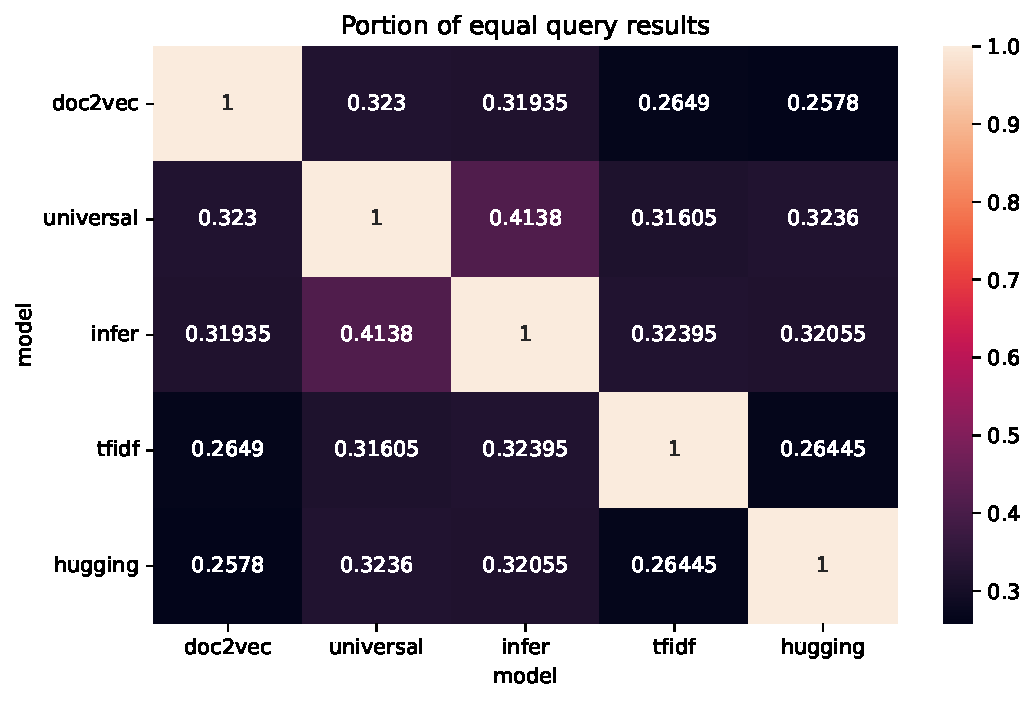
\includegraphics[width=0.7\textwidth]{images/comparison/Portion_of_equal_query_results.pdf}
    \caption[Comparison of models using a heatmap]
    {Heatmap visualizing portion of shared query results on 2000 queries à 10 responses on a 2048 document corpus.}
    \label{fig:heatmap-comparison-models}
\end{figure}

% heatmap interpretation
The heatmap in \autoref{fig:heatmap-comparison-models} shows that the models yield dissimilar query responses.
It arose from 2000 queries à 10 responses on a 2048 document corpus.
The similarity matrix was normalized to present the portion of shared query results for a query.
\ac{use} and \infersent{} produce the most similar responses, which indicates the maximum value of shared query results.
However, the maximum is less than $0.5$ and thus, rather dissimilar.
Any two-element combination of \ac{d2v}, \ac{tfidf} and \ac{sbert} produces the most dissimilar query results, 
namely only around $25\%$ of shared response documents per query.

% mean and std
Since the normalization does not consider the distribution of the cardinalities of the intersections of the query results among the models,
another approach is to calculate the mean and standard deviation of the cardinalities of the intersections of the query results.
Therefore, 30 trials were conducted.
Each trial consisted of 10 randomly sampled query documents à 10 responses (excluding the query document in the response).
The normalized similarity matrix for each model pair concerning one trial was calculated using \lst{lst:sim-matrix}.
The cardinalities were stored in a dictionary of lists indexed by the respective model pairs.
Finally, the mean and standard deviation were computed for each model pair and stored in a \ac{csv} file.
The results are displayed in \autoref{tab:mean_std_portion_shared_query_results}.
The standard deviation does not exceed $0.1$ for any model pair and is similar among all combinations.
As observed before, any two-element combination of \ac{d2v}, \ac{tfidf} and \ac{sbert} has the lowest mean portion ($18-20\%$) of shared query results.

\begin{table}[]
    \centering
    \caption{Mean and standard deviation of the average portion of shared response documents of different models on a 2048 document corpus.
    One trial produced five real values, i.e. one portion per model.
    A portion is obtained from 10 randomly sampled query documents à 10 responses (excluding the query document in the response).
    There were 30 trials.
    }
    \begin{tabular}{|l|l|l|l|}
    \hline
    \rowcolor[HTML]{C0C0C0} 
    \textbf{model 1} & \textbf{model 2} & \textbf{mean} & \textbf{std} \\ \hline
    \ac{d2v}          & \ac{use}        & 0.26          & 0.09         \\ \hline
    \ac{d2v}          & \infersent{}            & 0.26          & 0.07         \\ \hline
    \ac{d2v}          & \ac{tfidf}            & 0.2           & 0.08         \\ \hline
    \ac{d2v}          & \ac{sbert}          & 0.18          & 0.06         \\ \hline
    \ac{use}        & \infersent{}            & 0.33          & 0.08         \\ \hline
    \ac{use}        & \ac{tfidf}            & 0.25          & 0.08         \\ \hline
    \ac{use}        & \ac{sbert}          & 0.25          & 0.06         \\ \hline
    \infersent{}            & \ac{tfidf}            & 0.26          & 0.08         \\ \hline
    \infersent{}            & \ac{sbert}          & 0.24          & 0.06         \\ \hline
    \ac{tfidf}            & \ac{sbert}          & 0.18          & 0.05         \\ \hline
    \end{tabular}
    \label{tab:mean_std_portion_shared_query_results}
\end{table}



% sample query
To display the differences between the models exemplary, the five most similar documents to a random document were returned from the database and visualized.
The text of the query document was encoded using the respective model and a 
\ac{knn} query was used to obtain the results from the local database containing 2048 documents.
The query image, i.e. the one surrounded by a border, was omitted from the database query response.
The query responses are listed according to descending similarity to the query document.
The query results are displayed in \autoref{fig:query_resp}.
% \autoref{fig:query_resp_doc2vec} displays the \ac{d2v} reponses,  
% \autoref{fig:query_resp_sbert} displays the \ac{sbert} reponses,  
% \autoref{fig:query_resp_tfidf} displays the \ac{tfidf} reponses,  
% \autoref{fig:query_resp_infer} displays the \infersent{} reponses,  
% \autoref{fig:query_resp_use} displays the \ac{use} reponses.
All models except \ac{d2v} and \ac{use} returned only documents of \textit{CREDIT SUISSE}.
Apart from this difference, the query responses of the models are very similar.


% sample query
\begin{figure}[h!]
    \begin{subfigure}{\textwidth}
        \centering
        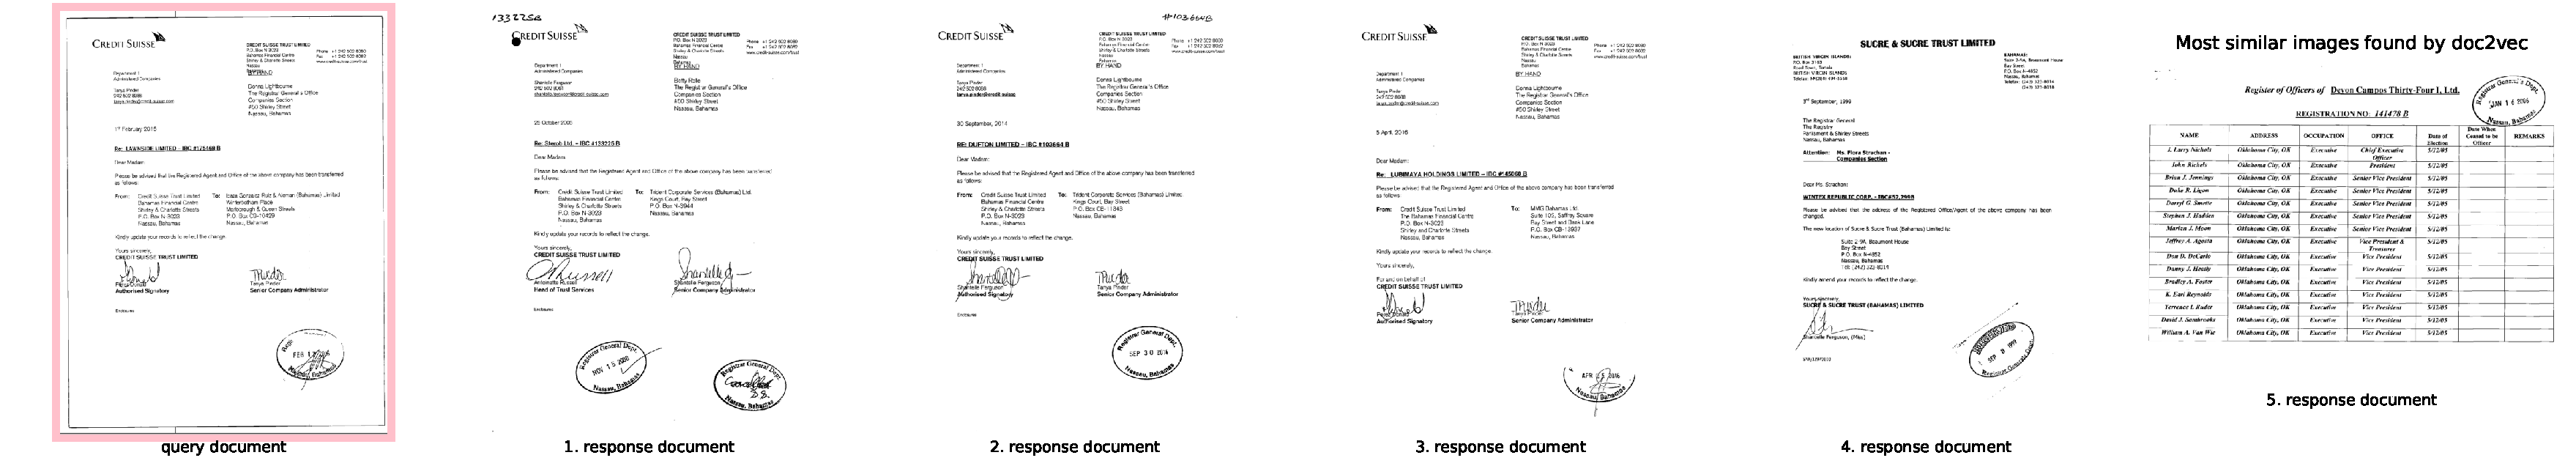
\includegraphics[width=1\textwidth]{images/query_results/4b4d0a9ee0c7283e5bfd69c402c73b2140bf90351c8f44d6809afe23c6dfaa50/Most_similar_images_found_by_doc2vec.pdf}
        \caption{\ac{d2v}}
        \label{fig:query_resp_doc2vec}
    \end{subfigure}

    \begin{subfigure}{\textwidth}
        \centering
        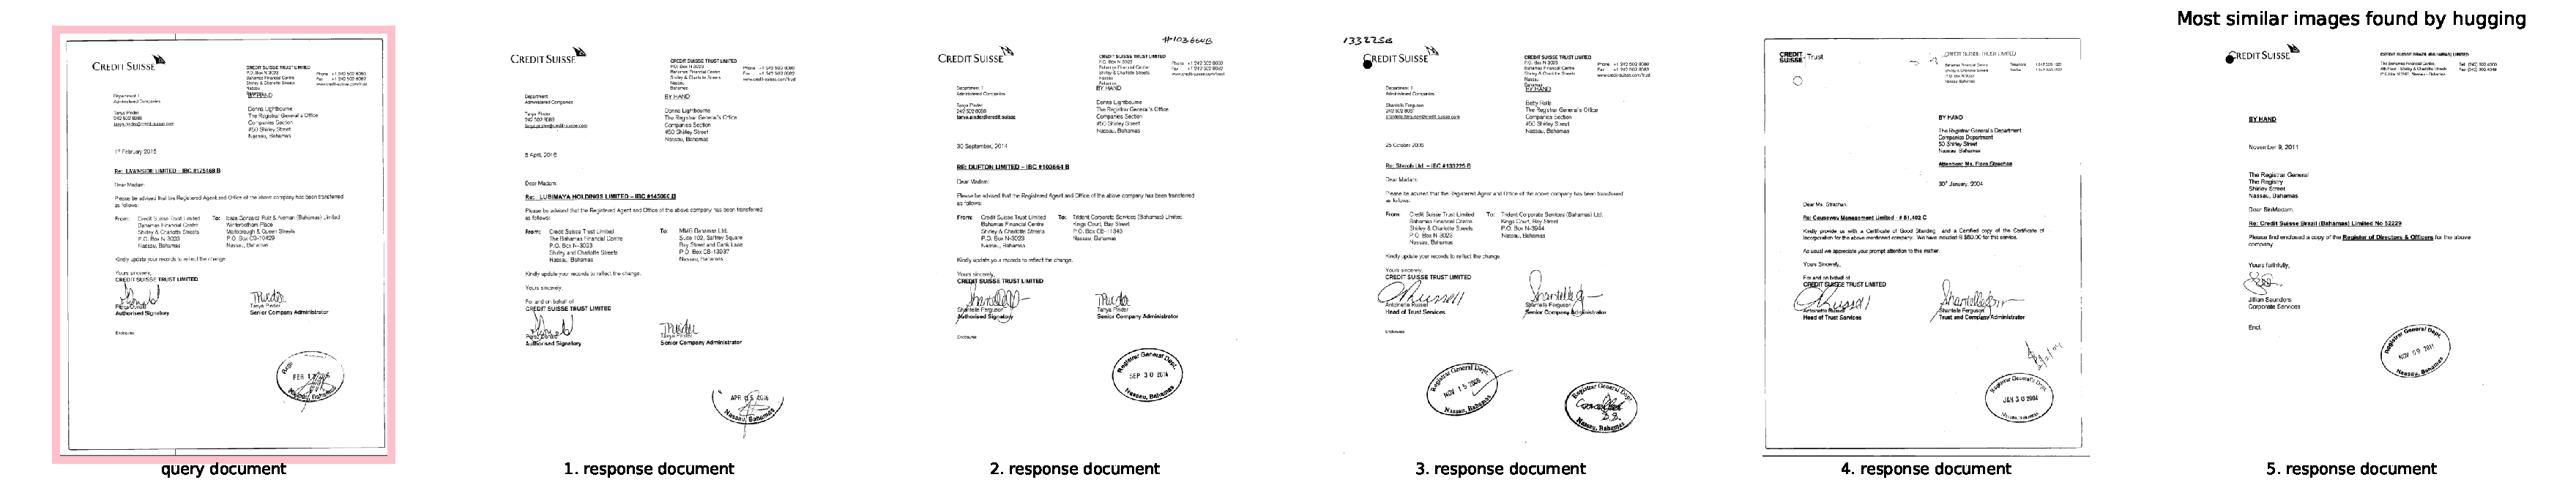
\includegraphics[width=1\textwidth]{images/query_results/4b4d0a9ee0c7283e5bfd69c402c73b2140bf90351c8f44d6809afe23c6dfaa50/Most_similar_images_found_by_hugging.pdf}
        \caption{\ac{sbert}}
        \label{fig:query_resp_sbert}
    \end{subfigure}

    \begin{subfigure}{\textwidth}
        \centering
        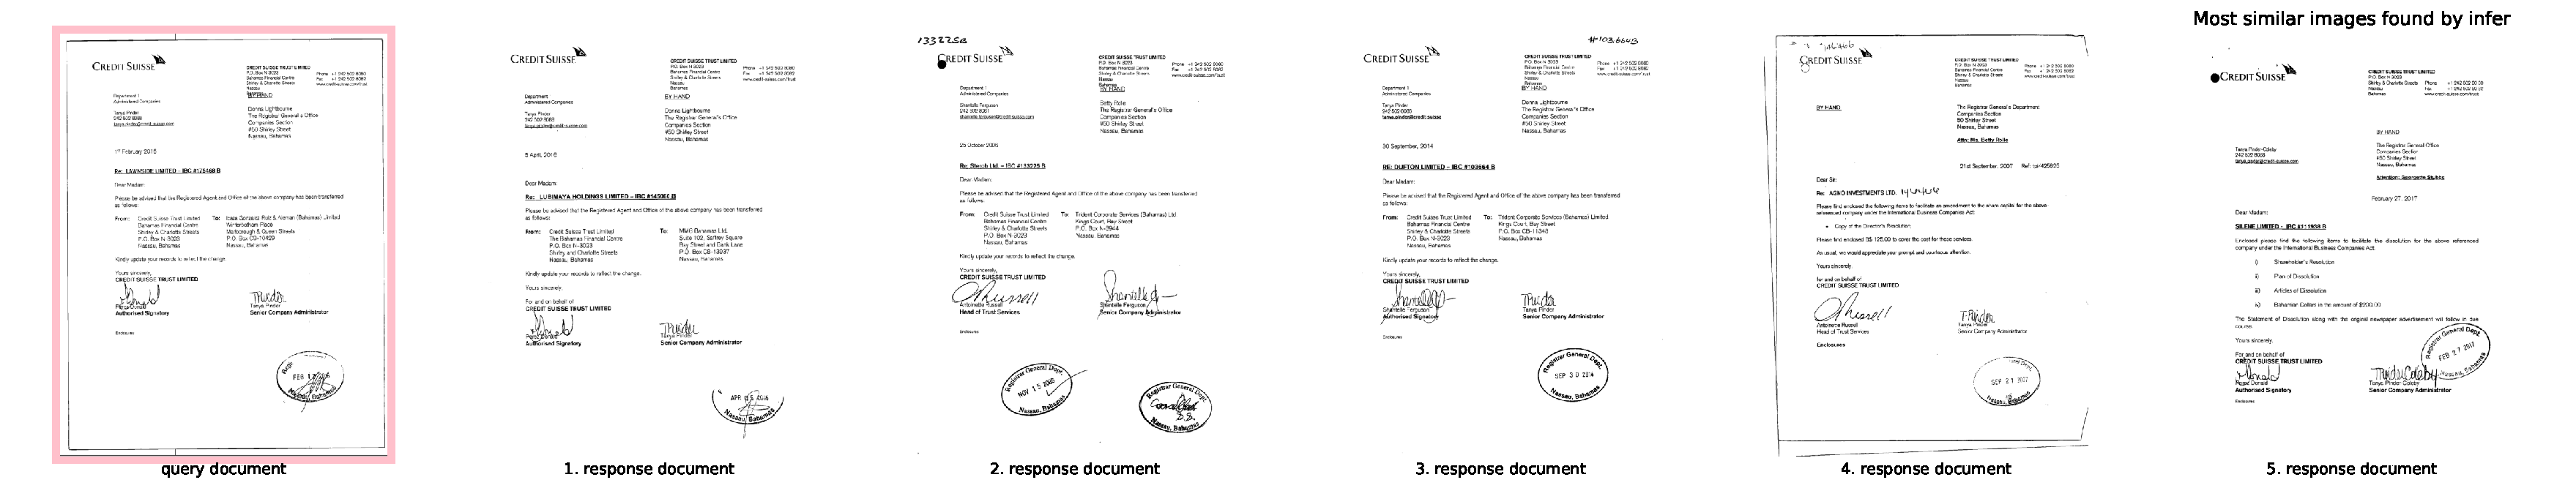
\includegraphics[width=1\textwidth]{images/query_results/4b4d0a9ee0c7283e5bfd69c402c73b2140bf90351c8f44d6809afe23c6dfaa50/Most_similar_images_found_by_infer.pdf}
        \caption{\infersent{}}
        \label{fig:query_resp_infer}
    \end{subfigure}

    \begin{subfigure}{\textwidth}
        \centering
        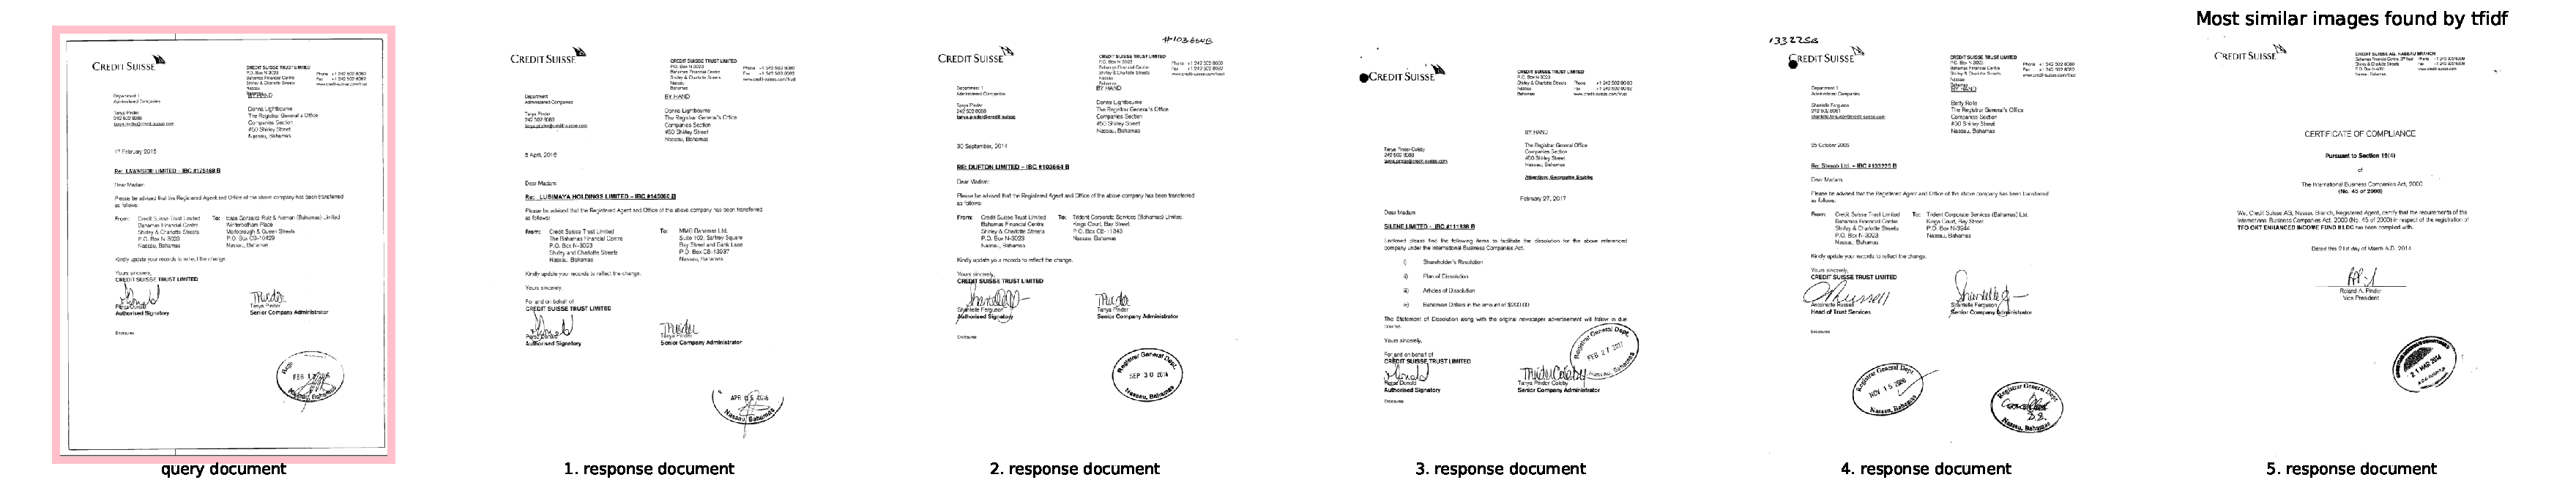
\includegraphics[width=1\textwidth]{images/query_results/4b4d0a9ee0c7283e5bfd69c402c73b2140bf90351c8f44d6809afe23c6dfaa50/Most_similar_images_found_by_tfidf.pdf}
        \caption{\ac{tfidf}}
        \label{fig:query_resp_tfidf}
    \end{subfigure}

    \begin{subfigure}{\textwidth}
        \centering
        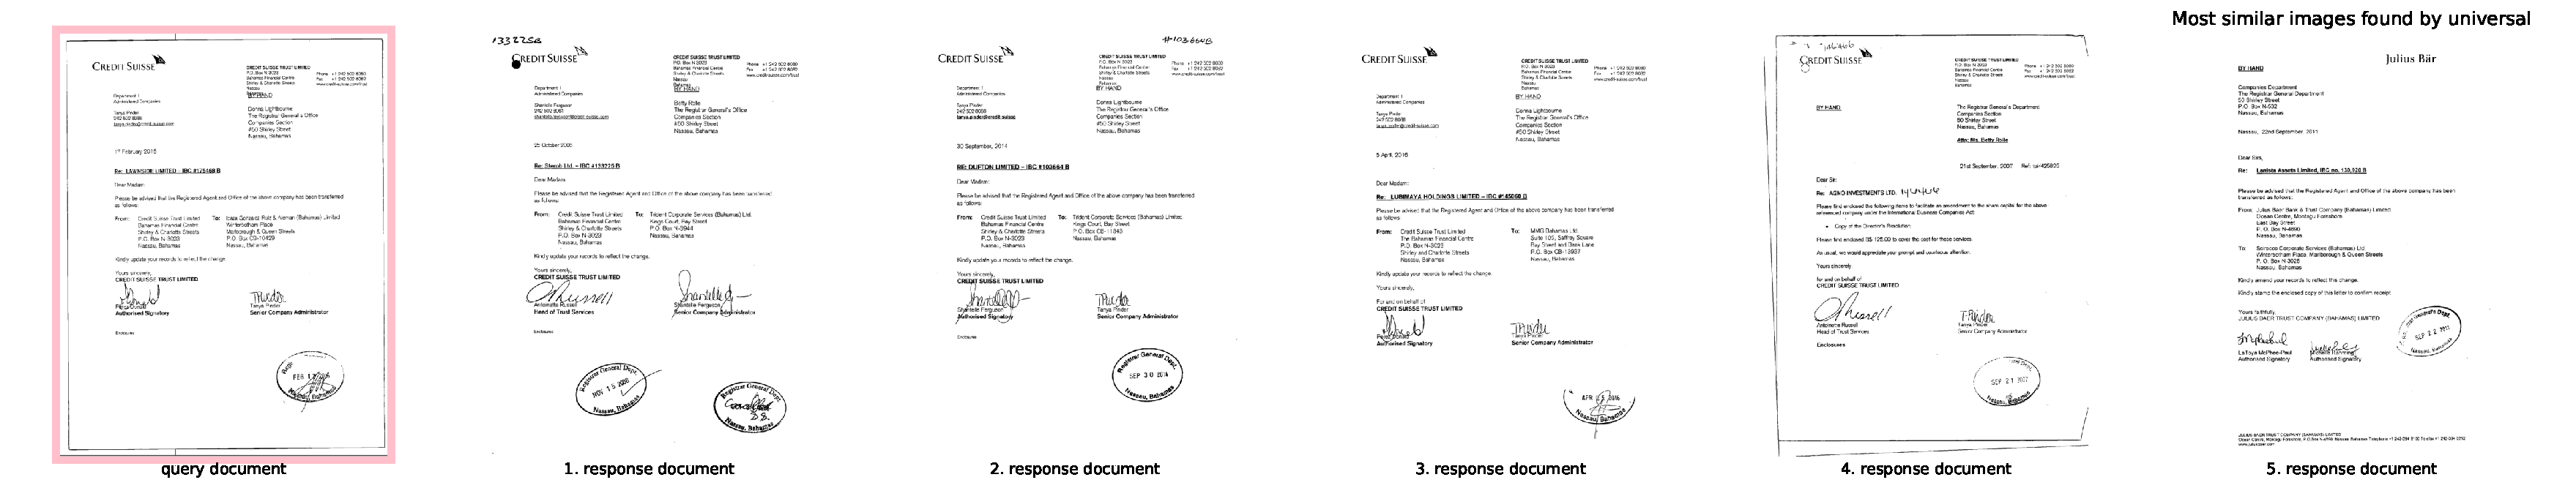
\includegraphics[width=1\textwidth]{images/query_results/4b4d0a9ee0c7283e5bfd69c402c73b2140bf90351c8f44d6809afe23c6dfaa50/Most_similar_images_found_by_universal.pdf}
        \caption{\ac{use}}
        \label{fig:query_resp_use}
    \end{subfigure}
\caption[Exemplary query response]{Exemplary query response for different embeddings on the same query document.}
\label{fig:query_resp}
\end{figure}

To further investigate the differences between the models, 
the query responses of the models are compared qualitatively on documents that were found to be unusual in terms of visual inspection.
The first document in \autoref{fig:comp_query_resp} is a table consisting of little text compared to other samples from the data corpus.
The second document in \autoref{fig:comp_query_resp} is mostly handwritten, which is unusual since most other samples are computer generated.

% good results
The models produced good query responses on a query document consisting of little text as shown in \autoref{fig:good_query_resp_infer}.
Even though at first glimpse, the response documents seem unrelated to the query document, they share multiple words, such as \textit{director}.
Similar response documents do not have to be of similar visual appearance since the text embeddings only consider information from the text layer.

\begin{figure}[!htb] % htp = hier (h), top (t), oder auf einer eigenen Seite (p).
    \centering
    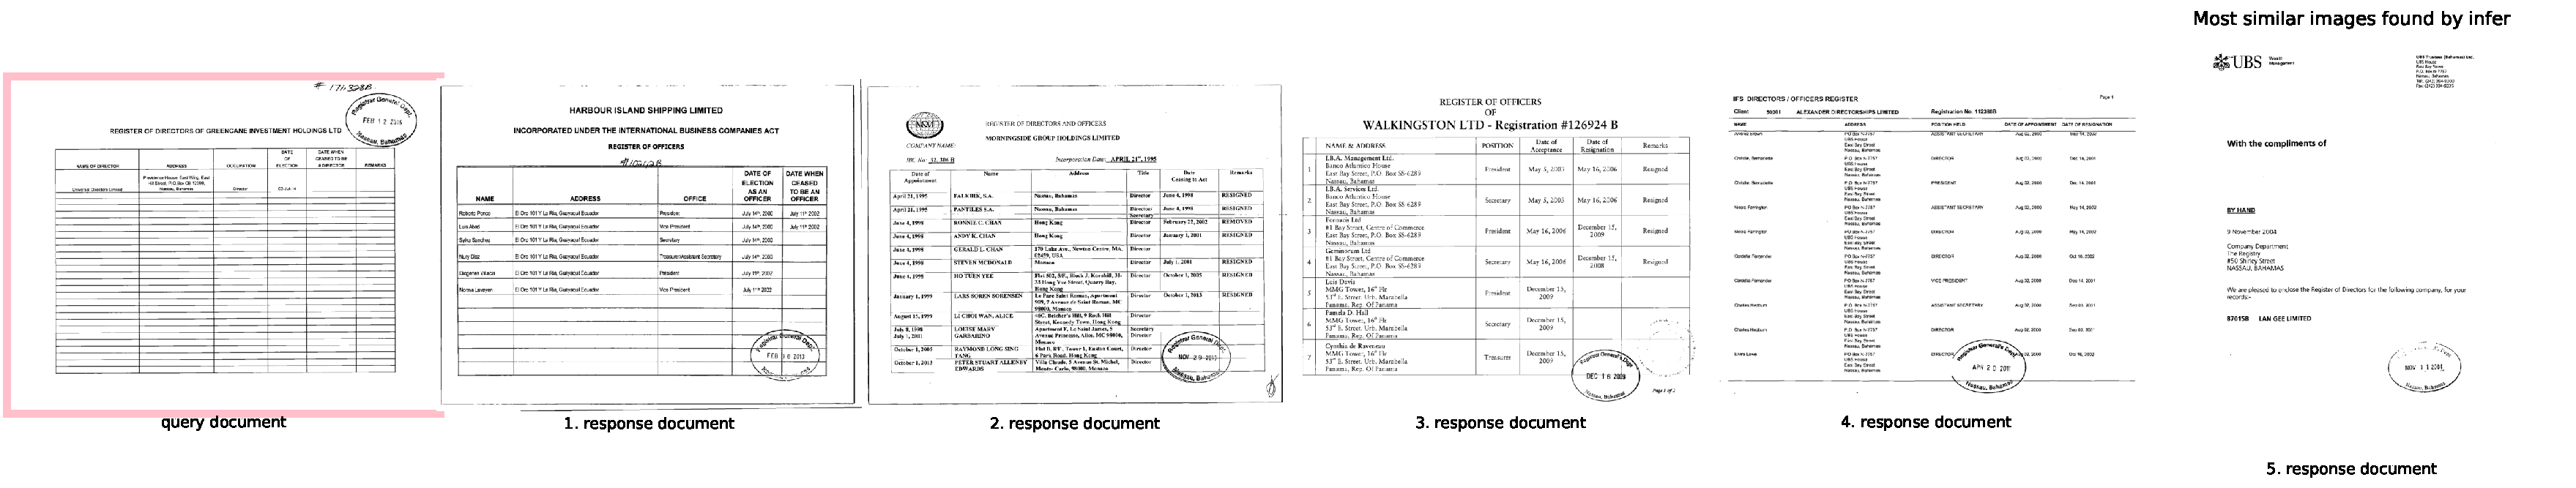
\includegraphics[width=1\textwidth]{images/query_results/42b7e56855c88c22ed01f381167e6f0887815e1ef7ea6b149be06ee1f8557b9e/Most_similar_images_found_by_infer.pdf}
    \caption[\infersent{} query responses]{\infersent{} query responses on a query document consisting of little text.
    }
    \label{fig:good_query_resp_infer}
\end{figure}

% bad results
There are query documents such as the one in \autoref{fig:comp_query_resp} that reveal the dissimilarity between certain models.
Most models' response documents are similar to \autoref{fig:good_query_resp_sbert}.
These response documents depict the same type of document, i.e. handwritten receipts for an annual fee.
The \ac{tfidf} model, however, returns different response documents.
The response documents from \autoref{fig:bad_query_resp_tfidf} are not handwritten and cover a different content, 
i.e. requesting a payment and three documents concerning an address change.
\ac{tfidf}'s results could thus be considered to be of poor quality.

\begin{figure}[h!]
    \ContinuedFloat
    \begin{subfigure}{\textwidth}
        \centering
        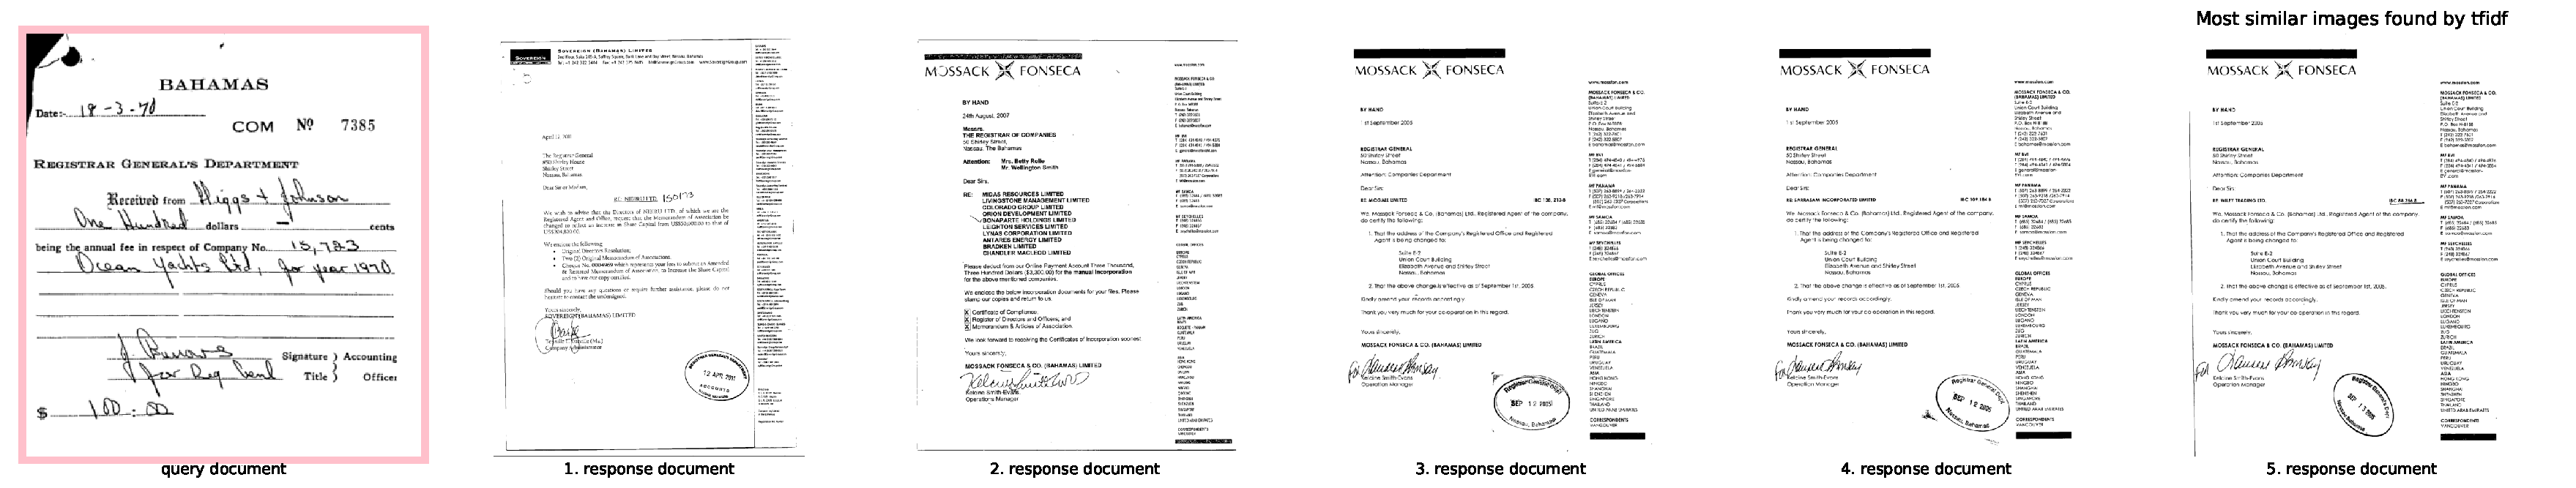
\includegraphics[width=1\textwidth]{images/query_results/4542b223317eba23e4bda3e1536d61c8e2d2890a6439830ca8c62650bc1aac70/Most_similar_images_found_by_tfidf.pdf}
        \caption{\ac{tfidf}}
        \label{fig:bad_query_resp_tfidf}
    \end{subfigure}

    \begin{subfigure}{\textwidth}
        \centering
        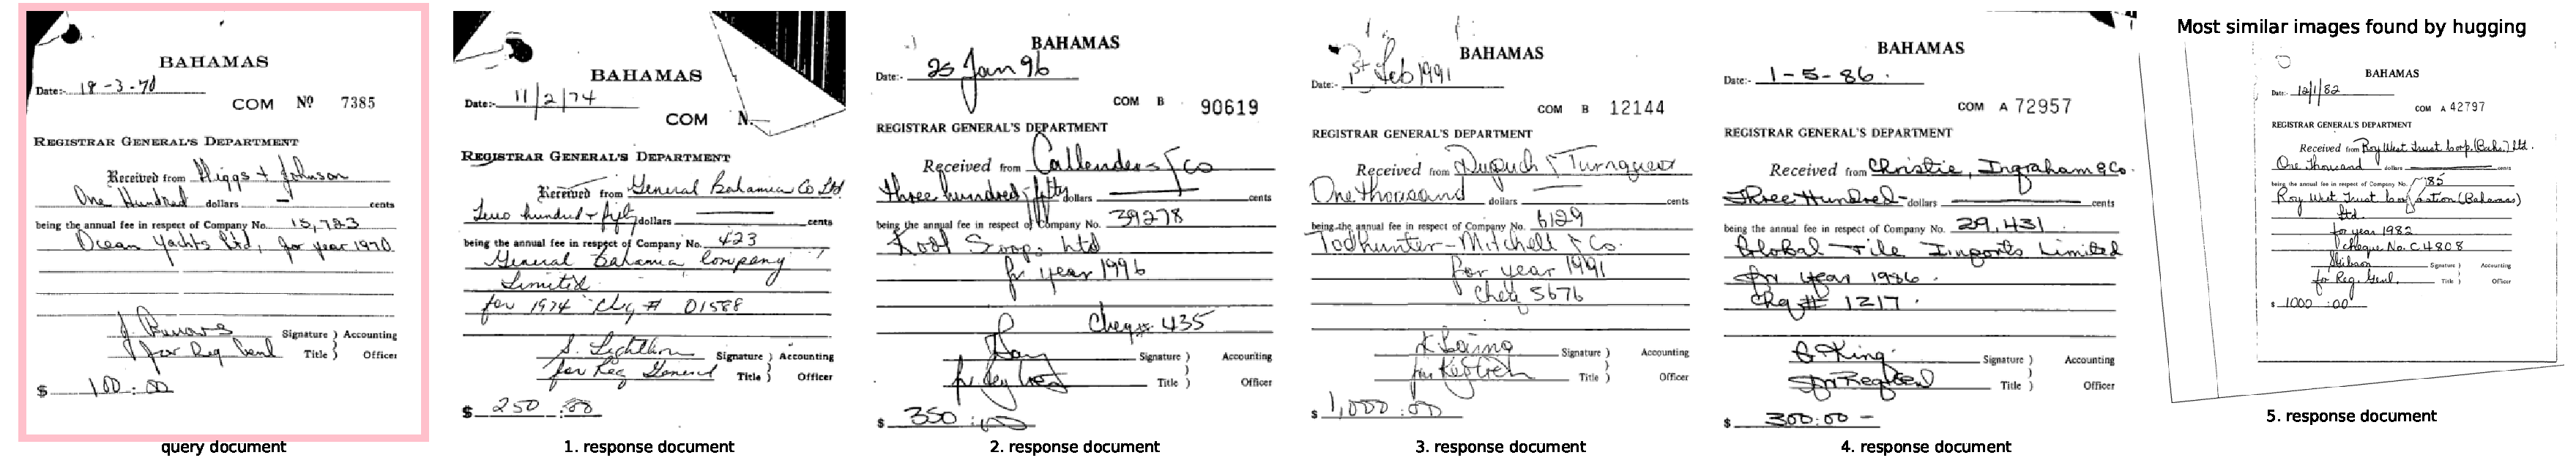
\includegraphics[width=1\textwidth]{images/query_results/4542b223317eba23e4bda3e1536d61c8e2d2890a6439830ca8c62650bc1aac70/Most_similar_images_found_by_hugging.pdf}
        \caption{\ac{sbert}}
        \label{fig:good_query_resp_sbert}
    \end{subfigure}

\caption[Qualitative comparison of query responses]{Qualitative comparison of query responses.
The majority of the query document consists of handwritten text.
The results of the \ac{tfidf} model are not very similar to the query document and thus, are considered to be of poor quality.
The other models, for example, \ac{sbert}, produce results that are more similar to the query document.
}
\label{fig:comp_query_resp}
\end{figure}

% visual vs. textual similarity
Since not only textual information but also visual information is encoded in the database, 
the next step is to compare the query responses of approaches that consider visual similarity.
The query responses are clustered using \ac{optics} or \texttt{argmax} of the \ac{pca} compression.

The first exemplary query document in \autoref{fig:comp_vis_query_resp} is an image of a usual document.
Both clustering approaches yield similar results.
More specifically, the responses share two documents.
Moreover, the last document in the response of both approaches differs most from the group.
None of the result documents originate from the same company as the query document.

The second exemplary query document in \autoref{fig:comp_vis_query_resp_certificates} is a certificate.
\ac{optics} clustering approach yields a response that is more similar to the query document than the \texttt{argmax} of the \ac{pca} compression
because all its responses are from the same document type as the query document.
Hence, the \ac{optics} clustering approach is considered to be superior to the \texttt{argmax} approach.

\begin{figure}[h!]
    \begin{subfigure}{\textwidth}
        \centering
        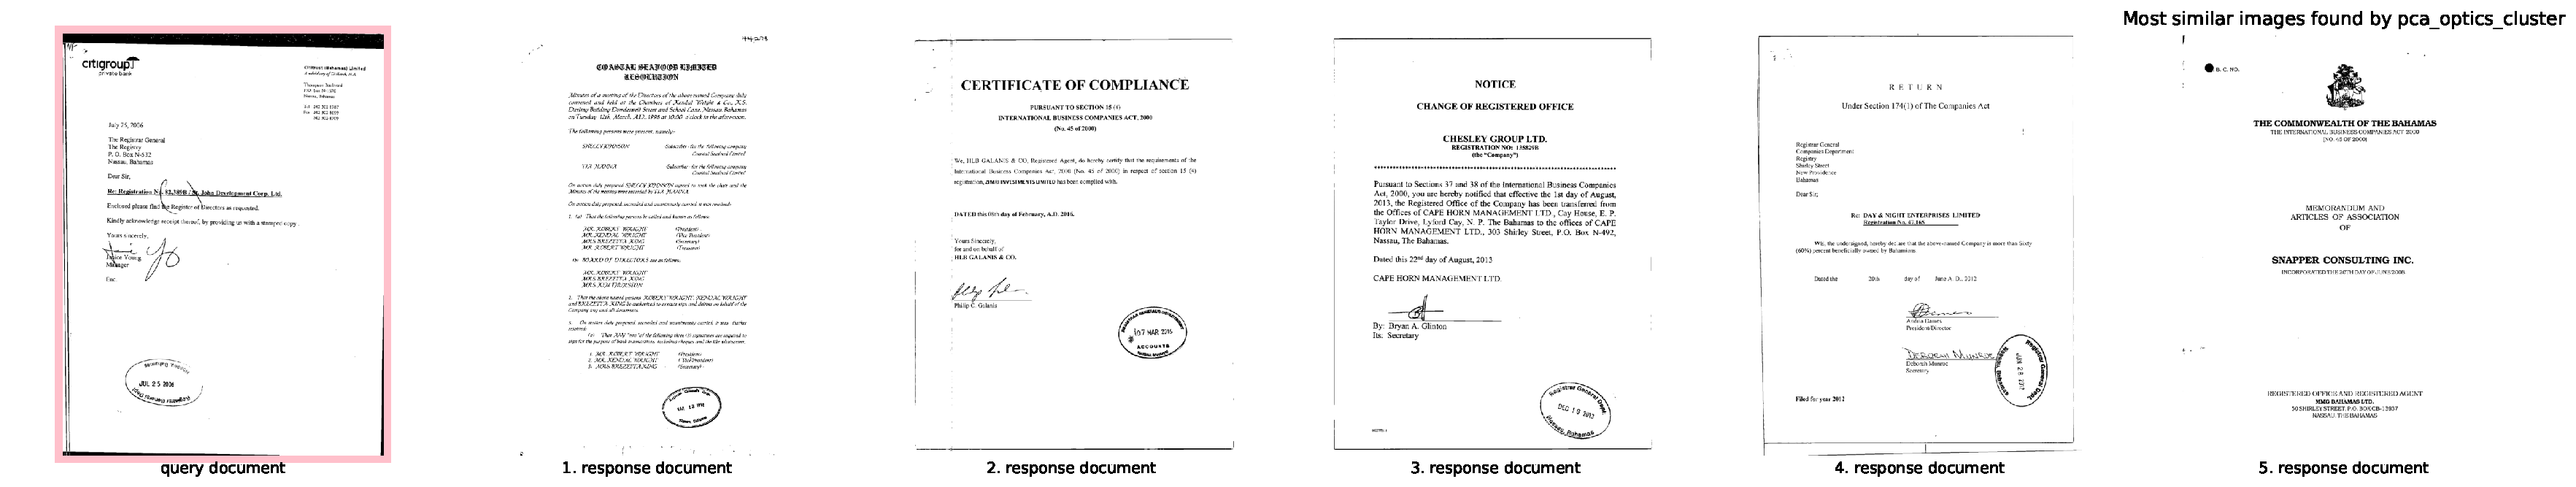
\includegraphics[width=1\textwidth]{images/query_results/d5b16dcfc7c090c1c0ea7503d3fce417a84aa429a078478fdb4291805fee1328/Most_similar_images_found_by_pca_optics_cluster.pdf}
        \caption{\ac{optics}}
        \label{fig:bad_query_resp_tfidf}
    \end{subfigure}

    \begin{subfigure}{\textwidth}
        \centering
        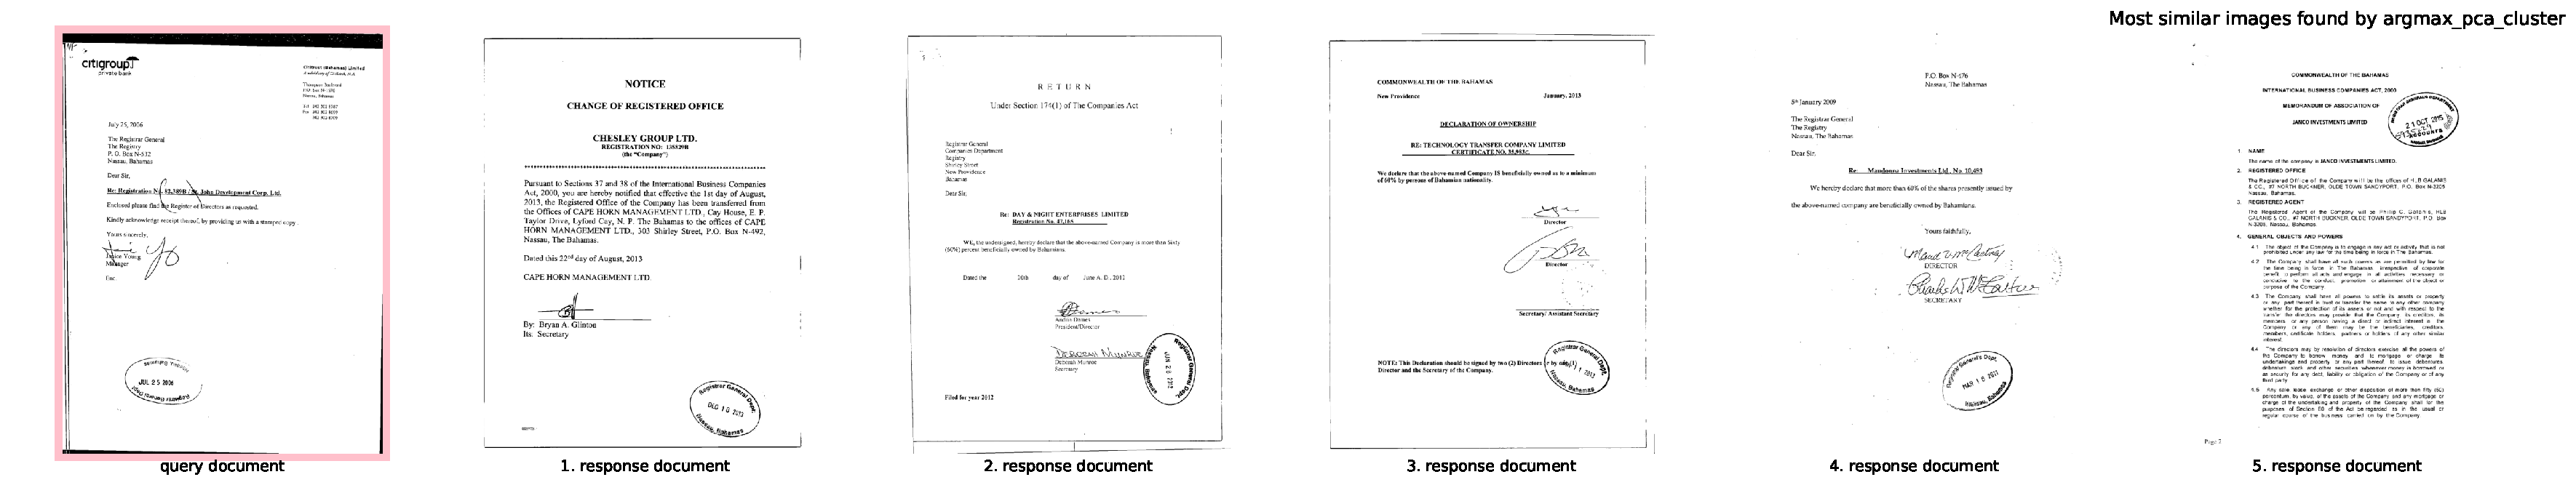
\includegraphics[width=1\textwidth]{images/query_results/d5b16dcfc7c090c1c0ea7503d3fce417a84aa429a078478fdb4291805fee1328/Most_similar_images_found_by_argmax_pca_cluster.pdf}
        \caption{\texttt{argmax} of \ac{pca} compression}
        \label{fig:good_query_resp_sbert}
    \end{subfigure}

\caption[Qualitative comparison of clustering on visual information]{Qualitative comparison of query responses.
The response documents are clustered using \ac{optics} or \texttt{argmax} of the \ac{pca} compression.
They are not compared in terms of textual but visual similarity.
}
\label{fig:comp_vis_query_resp}
\end{figure}

\begin{figure}[h!]
    \begin{subfigure}{\textwidth}
        \centering
        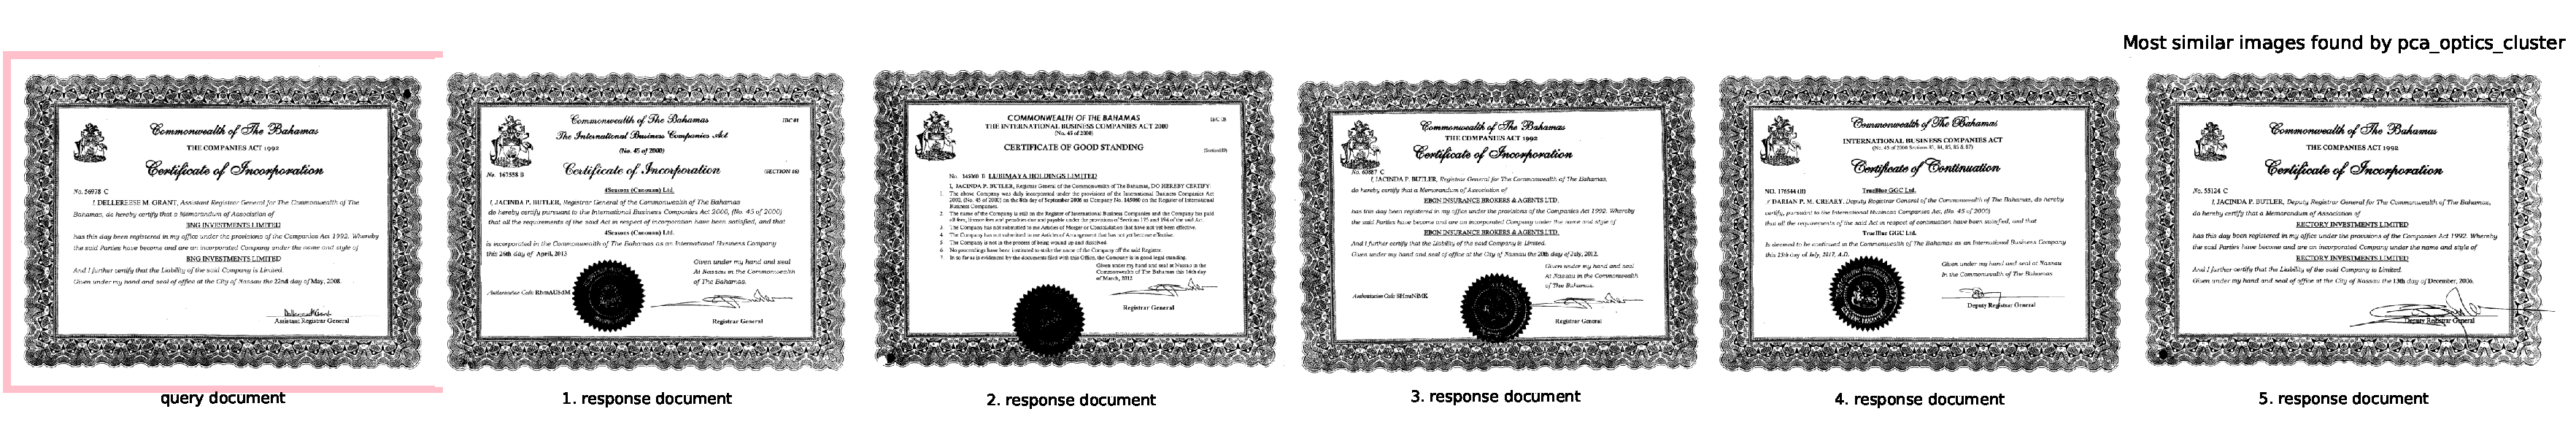
\includegraphics[width=1\textwidth]{images/query_results/320a70609babe5923c860ad16bc9f48e237b9d275c5269d177befab542bcff50/Most_similar_images_found_by_pca_optics_cluster.pdf}
        \caption{\ac{optics}}
        \label{fig:bad_query_resp_tfidf}
    \end{subfigure}

    \begin{subfigure}{\textwidth}
        \centering
        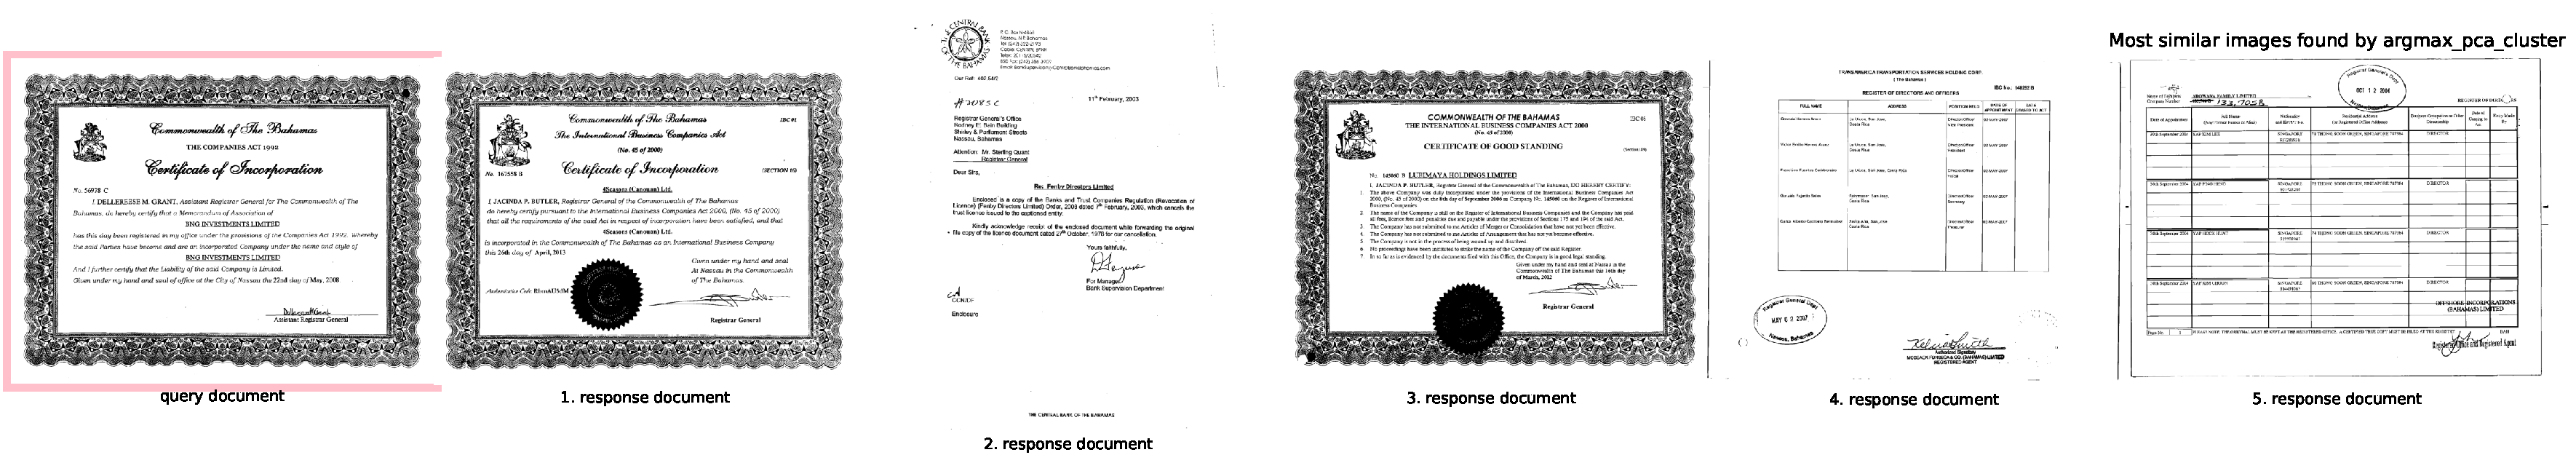
\includegraphics[width=1\textwidth]{images/query_results/320a70609babe5923c860ad16bc9f48e237b9d275c5269d177befab542bcff50/Most_similar_images_found_by_argmax_pca_cluster.pdf}
        \caption{\texttt{argmax} of \ac{pca} compression}
        \label{fig:good_query_resp_sbert}
    \end{subfigure}

\caption[Qualitative comparison of query responses]{Qualitative comparison of query responses.
The response documents are clustered using \ac{optics} or \texttt{argmax} of the \ac{pca} compression.
They are not compared in terms of textual but visual similarity.
The query document is a certificate.
}
\label{fig:comp_vis_query_resp_certificates}
\end{figure}